%%%%%%%%%%%%%%%%%%%%%%%%%%%%%%%%%%%%%%%%%
% Journal Article
% LaTeX Template
% Version 1.4 (15/5/16)
%
% This template has been downloaded from:
% http://www.LaTeXTemplates.com
%
% Original author:
% Frits Wenneker (http://www.howtotex.com) with extensive modifications by
% Vel (vel@LaTeXTemplates.com)
%
% License:
% CC BY-NC-SA 3.0 (http://creativecommons.org/licenses/by-nc-sa/3.0/)
%
%%%%%%%%%%%%%%%%%%%%%%%%%%%%%%%%%%%%%%%%%

%----------------------------------------------------------------------------------------
%	PACKAGES AND OTHER DOCUMENT CONFIGURATIONS
%----------------------------------------------------------------------------------------

\documentclass[twoside,twocolumn]{article}

\usepackage{blindtext} % Package to generate dummy text throughout this template 

\usepackage[sc]{mathpazo} % Use the Palatino font
\usepackage[T1]{fontenc} % Use 8-bit encoding that has 256 glyphs
\linespread{1.05} % Line spacing - Palatino needs more space between lines
\usepackage{microtype} % Slightly tweak font spacing for aesthetics

\usepackage[english]{babel} % Language hyphenation and typographical rules

\usepackage[hmarginratio=1:1,top=32mm,columnsep=20pt]{geometry} % Document margins
\usepackage[hang, small,labelfont=bf,up,textfont=it,up]{caption} % Custom captions under/above floats in tables or figures
\usepackage{booktabs} % Horizontal rules in tables

\usepackage{lettrine} % The lettrine is the first enlarged letter at the beginning of the text

\usepackage{enumitem} % Customized lists
\setlist[itemize]{noitemsep} % Make itemize lists more compact

\usepackage{abstract} % Allows abstract customization
\renewcommand{\abstractnamefont}{\normalfont\bfseries} % Set the "Abstract" text to bold
\renewcommand{\abstracttextfont}{\normalfont\small\itshape} % Set the abstract itself to small italic text

\usepackage{titlesec} % Allows customization of titles
\renewcommand\thesection{\Roman{section}} % Roman numerals for the sections
\renewcommand\thesubsection{\roman{subsection}} % roman numerals for subsections
\titleformat{\section}[block]{\large\scshape\centering}{\thesection.}{1em}{} % Change the look of the section titles
\titleformat{\subsection}[block]{\large}{\thesubsection.}{1em}{} % Change the look of the section titles

%\usepackage{fancyhdr} % Headers and footers
%\pagestyle{fancy} % All pages have headers and footers
%\fancyhead{} % Blank out the default header
%\fancyfoot{} % Blank out the default footer
%\fancyhead[C]{Running title $\bullet$ May 2016 %$\bullet$ Vol. XXI, No. 1} % Custom header text
%\fancyfoot[RO,LE]{\thepage} % Custom footer text

\usepackage{titling} % Customizing the title section

\usepackage[hidelinks]{hyperref} % For hyperlinks in the PDF
\usepackage{graphicx}
\graphicspath {{C:/Users/Miguel/Downloads/ Circuitos electronicos/}}
%----------------------------------------------------------------------------------------
%	TITLE SECTION
%----------------------------------------------------------------------------------------

\setlength{\droptitle}{-4\baselineskip} % Move the title up

\pretitle{\begin{center}\Huge\bfseries} % Article title formatting
\posttitle{\end{center}} % Article title closing formatting

\def\abstract
   {%
   \leftline{\normalsize \bf Abstract - }%
   \bf\small
   }

\def\endabstract
   {
   % additional empty line at the end of the abstract
   \vspace*{0.1in}% What about 1em instead?%
   }

\title{Experimento N°1\\Mediciones en Circuitos DC} % Article title
\author{%x  x
\textsc{William Guadalupe}\textsc{, Miguel Roca}\textsc{, Jesús Marin}\\
%\thanks{A thank you or further information} \\[1ex] % Your name
\normalsize Facultad de Ciencias \\ % Your institution
\normalsize Universidad Nacional de Ingenieria \\ % Your institution
\normalsize \href{mailto:wguadalupeq@uni.pe}{wguadalupeq@uni.pe},  \href{mailto:miguel.roca.a@uni.pe}{miguel.roca.a@uni.pe} \href{mailto:john@smith.com}{,  john3@smith.com} % Your email address
%\and % Uncomment if 2 authors are required, duplicate these 4 lines if more
%\textsc{Jane Smith}\thanks{Corresponding author} \\[1ex] % Second author's name
%\normalsize University of Utah \\ % Second author's institution
%\normalsize \href{mailto:jane@smith.com}{jane@smith.com} % Second author's email address
}
%\date{\today} % Leave empty to omit a date
\date{ }
\renewcommand{\maketitlehookd}{%
%\begin{abstract}
%\noindent \blindtext % Dummy abstract text - %replace \blindtext with your abstract text
%\end{abstract}
}

%----------------------------------------------------------------------------------------

\begin{document}

% Print the title
\maketitle

%----------------------------------------------------------------------------------------
%	ARTICLE CONTENTS
%----------------------------------------------------------------------------------------
\begin{abstract}

En este experimento tomaremos medidas, usando el sofware Multisim, en circuitos resistivos simples usando un multimetro digital con el fin de comprobar la ley de ohm y hallar los posibles errores de medicion que se producen en la realidad. Se encontro que los errores de medicion mayormente se producen debido a que las resistencias internas del voltimetro o del amperimetro deben ser lo mas cerca al valor teorico (ideal) por eso se deberia tomar en cuenta las resistencias internas de los aparatos dependiendo del circuito en el cual se trabajara.

\end{abstract}

\section{Introducción}
El uso de los aparatos electrónicos se ha extendido exponencialmente en los últimos años, gracias a los rápidos avances de la tecnología. Mediante este experimento, lograremos estudiar algunos de sus componentes esenciales, así como los procesos que los envuelven.\\

\textbf{Fundamento Teórico}
\begin {itemize}
\item Resistencia: la oposición al flujo de corriente eléctrica a través de un conductor.
\item Potenciómetro: resistencia variable mecánica.
\item Corriente continua: flujo continuo de carga eléctrica a través de un conductor entre dos puntos de distinto potencial y carga eléctrica, que no cambia de sentido con el tiempo
\item Diferencia de potencial: es una magnitud física que cuantifica la diferencia de potencial eléctrico entre dos puntos.
\item Amperímetro: galvanómetro que mide la intensidad de corriente eléctrica.
\item Voltímetro: galvanómetro que mide la diferencia de potencial entre dos puntos.
\item Circuito eléctrico:  interconexión de componentes eléctricos que transporta la corriente eléctrica a través de una trayectoria cerrada.
\item Ley de Ohm: Establece que la diferencia de potencial V que aplicamos entre los extremos de un conductor determinado es directamente proporcional a la intensidad de la corriente I que circula por el citado conductor. V= IR.
\end{itemize}

%------------------------------------------------

\section{Objetivos generales y especificos}

\textbf{Objetivo General} 
\begin{itemize}
\item Realizar mediciones eléctricas en circuitos resistivos simples usando el multímetro digital, identificando errores de medición y considerando la impedancia del instrumento de medición.
\end{itemize}

\textbf{Objetivos Específicos}

\begin{itemize}
\item Comprender, analizar y diseñar el circuito divisor de voltaje.
\item Comprobar el comportamiento de la impedancia del voltímetro.
\item Comprender, analizar y diseñar el circuito divisor de corriente.
\item Comprobar el comportamiento de la impedancia del amperímetro.
\end{itemize}


%------------------------------------------------
%\newpage
\section{Datos Tabulados}
\begin{itemize}
\item Paso 1: Medición de resistencias, codigo de colores.
\\
\textbf{a)Resistencias de 4 y 5 bandas}
\begin{table}[h]
    \centering
    \scalebox{0.6}{
    \begin{tabular}{|c|c|c|c|c|} \hline
      Colores & R nominal  & Tolerancia(\%)  & \triangle R  &  R \pm \triangle R \\ \hline
       Rojo,amarillo & 24k\Omega  & \pm 2  & \pm 480\Omega  & 24 \pm 480 \Omega \\ 
       naranja,rojo  & & & & \\ \hline
       Amarillo, azul & 460\Omega  & \pm 5  & \pm 23\Omega  & 460 \pm 23 \Omega \\ 
       marrón , dorado  & & & & \\ \hline       
        violeta,negro  & 7000k\Omega  & \pm 10  & \pm 700k\Omega  & 7000 \pm 700k \Omega \\ 
        verde , plateado  & & & & \\ \hline       
        amarillo, rojo  & 420k\Omega  & \pm 0.25  & \pm 1.05k\Omega  & 420 \pm 1.05k \Omega \\
        negro,naranja,azul  & & & & \\ \hline       
        Verde,gris  & 5890\Omega  & \pm 1  & \pm 58.9\Omega  & 5890 \pm 58.9 \Omega \\ 
        blanco,marrón, marrón  & & & & \\ \hline       
    \end{tabular}
    }
    \caption{Medición de resistencias}
    \label{tab:tabla de resistencia}
\end{table}


\textbf{ b)Calculo de resistencia equivalente entre a y c, medir $R_{ac}$}

\textbf{considerar R=15\ohm}

\begin{table}[h]
\centering
\scalebox{0.8}{
    \begin{tabular}{|c|c|} \hline
      R medido & R calculado \\ \hline
      10 \Omega  & 10 \Omega \\ \hline
    \end{tabular}
    
}
    \caption{Resistencia equivalente}
    \label{tab:resistenciaequivalente}
\end{table}\\

\item Paso 2: Diseño de un divisor de voltaje
\enlargethispage{100mm}
\begin{table}[h]
\centering
\scalebox{0.8}{
    \begin{tabular}{|c|c|c|} \hline
      V_{BC}/V_{AC} & R2  & V_{BC}/V_{AC} medido \\ \hline
        1/2 & 10 KV & 1/2   \\ \hline
        1/4 & 5 KV & 1/4  \\ \hline
    \end{tabular}
}
    \caption{Relacion de voltajes en puntos BC y AC}
    \label{tab:tabla de resistencia}
\end{table}
\newpage
$R1=10 K\Omega$
\begin{table}[h]
\centering
\scalebox{1}{
    \begin{tabular}{|c|c|c|} \hline
      R_{x} & V_{x}  & I \\ \hline
      10 \%  & 909.09 mV & 909.09 $\mu A$  \\ \hline
      25 \%  & 2 V & 799.998 $\mu A$  \\ \hline
      35 \%  & 2.593 V & 740.739 $\mu A$  \\ \hline
      40 \%  & 2.857 V & 714.284 $\mu A$  \\ \hline
      60 \%  & 3.75 V & 624.998 $\mu A$  \\ \hline
    \end{tabular}
}
    \caption{Variación de la resistencia del potenciómetro $R1=10 K\Omega$}
    \label{tab:tabla de resistencia}
\end{table}
\newline
$R1=10 M\Omega$
\begin{table}[h]
\centering
\scalebox{1}{
    \begin{tabular}{|c|c|c|} \hline
      R_{x} & V_{x}  & I \\ \hline
      10 \%  & 999.904 uV & 999.889 $\mu A$  \\ \hline
      25 \%  & 2.499 mV & 999.756 $\mu A$  \\ \hline
      35 \%  & 3.499 mV & 999.645 $\mu A$  \\ \hline
      40 \%  & 3.998 mV & 999.6 $\mu A$  \\ \hline
      60 \%  & 5.996 mV & 999.401 $\mu A$  \\ \hline
    \end{tabular}
}
    \caption{Variación de la resistencia del potenciómetro $R1=10 M\Omega$}
    \label{tab:tabla de resistencia}
\end{table}

\item Paso 3: Impedancia del voltimetro y mediciones de voltaje.
\begin{table}[h]
\centering
\scalebox{0.8}{
    \begin{tabular}{|c|c|c|c|} \hline
      R_{1},R_{2} & V_{BC}(V) esperado  & V_{BC}(V) medido  & \% error relativo  \\ \hline
       10 K\Omega & 5 V & 4.998 V  & 0.04 \%  \\ \hline
       1 M\Omega& 5 V & 4.762 V  & 4.76 \%  \\ \hline
       10 M\Omega& 5 V & 3.333 V  & 33.34 \%  \\ \hline
    \end{tabular}
}
    \caption{Cálculo del voltaje para resistencias cercanas a la resistencia interna del voltimetro}
    \label{tab:tabla de resistencia}
\end{table}

\newpage
\item Paso 4: Diseño de un divisor de corriente
\begin{table}[h]
\centering
\scalebox{0.8}{
    \begin{tabular}{|c|c|c|} \hline
      I_{2}/I & R calculado  & I_{2}/I (medido)  \\ \hline
       1/2 & R_{2}= 10 K\Omega & 1/2   \\ \hline
       1/4 & R_{3}= 5 K\Omega & 1/4   \\ \hline
    \end{tabular}
}
    \caption{Relación de intensidad entre $I_{1}$ e $I_{2}$}
    \label{tab:tabla de resistencia}
\end{table}


\item Paso 5: Impedancia del amperimetro y mediciones de corriente.\\
Considerando amperimetro ideal, $I_{calculado}=I_{0}= 1 mA$

\begin{table}[h]
\centering
\scalebox{0.8}{
    \begin{tabular}{|c|c|c|} \hline
       & I_{medido}  & \% error relativo \\ \hline
        R_{A}= 100 \Omega & 990.099 $\mu A$  & 0.9901 \%  \\ \hline
        R_{A}= 20 \Omega & 998.004 $\mu A$  & 0.1996 \%  \\ \hline
    \end{tabular}
}
    \caption{Cálculo de la impedancia del amperimetro}
    \label{tab:tabla de resistencia}
\end{table}
\\
\end{itemize}

\section{Cálculos, gráficos y resultados}

\begin{itemize}
\item Simulación del paso 1
    \begin{figure}[h]
    \centering
    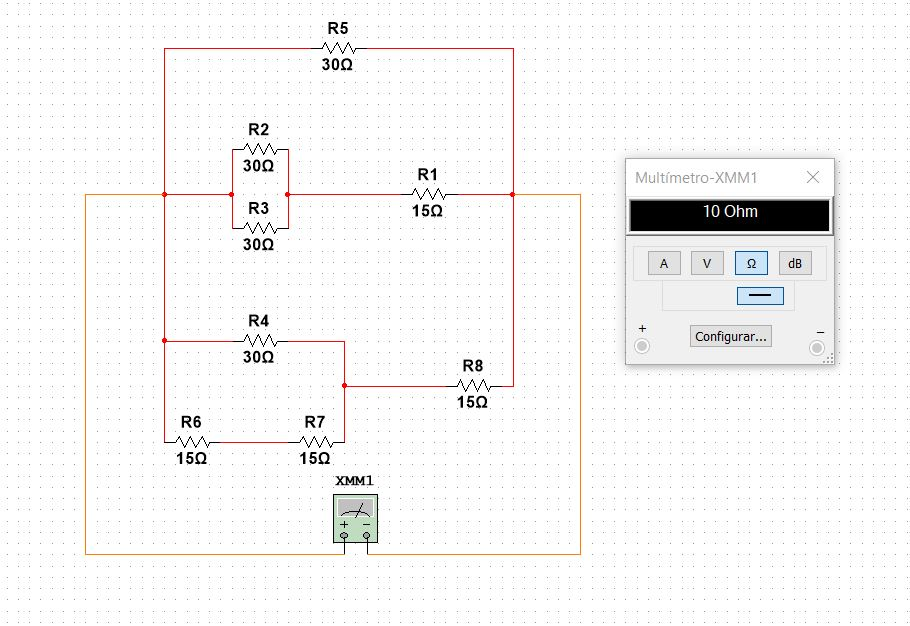
\includegraphics[scale=0.45]{imagenes1/1.b.JPG}
    \caption{Resistencia equivalente}
    \label{fig:circuito1}
    \end{figure}
\newpage    
\item Simulación del paso 2
    \begin{figure}[h]
    \centering
    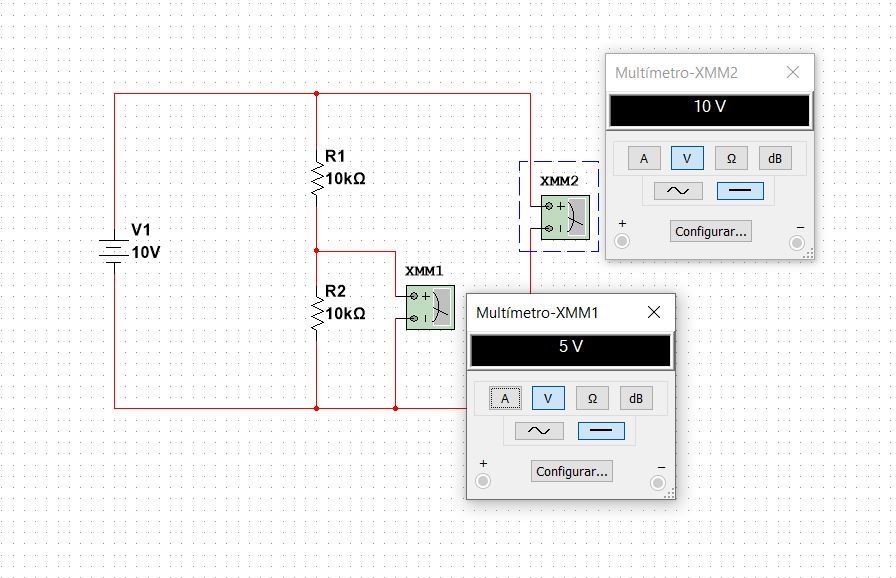
\includegraphics[scale=0.3]{imagenes1/2.1.JPG}
    \caption{Voltaje en BC y AC para $R_{1}$=10 K$\Omega$ y $R_{2}$=10 K$\Omega$}
    \label{fig:circuito1}
    \end{figure}
    
    \begin{figure}[h]
    \centering
    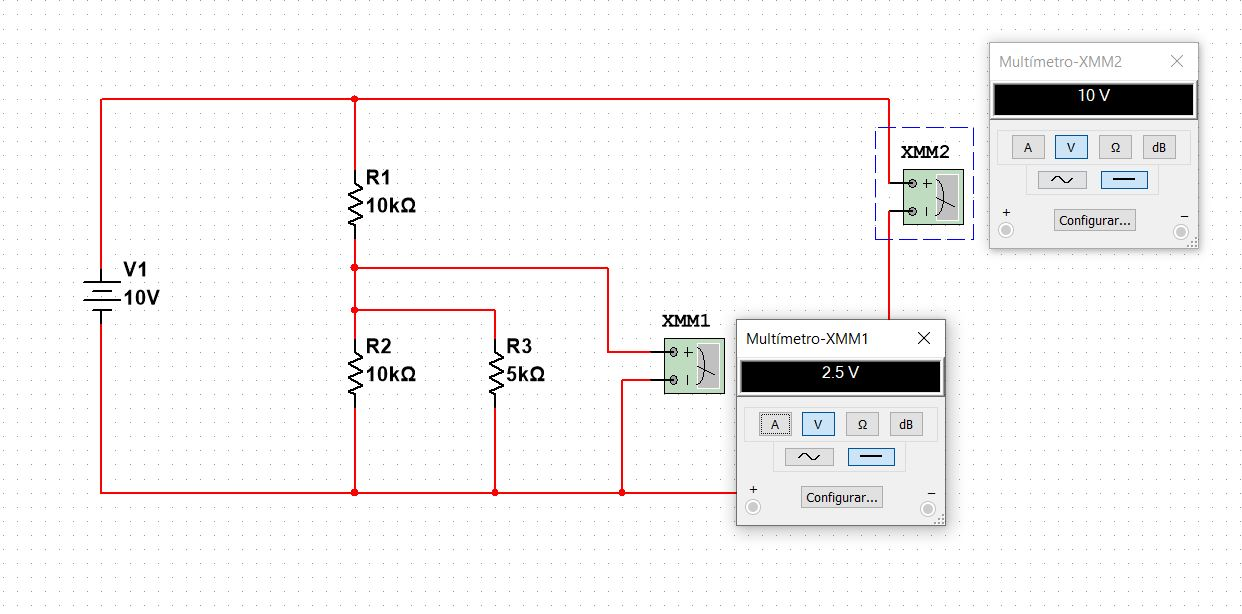
\includegraphics[scale=0.28]{imagenes1/2.2.JPG}
    \caption{Voltaje en BC y AC para $R_{1}$=10 K$\Omega$ , $R_{2}$=10 K$\Omega$ y $R_{3}$=5 K$\Omega$}
    \label{fig:circuito2}
    \end{figure}
    
    \begin{figure}[h]
    \centering
    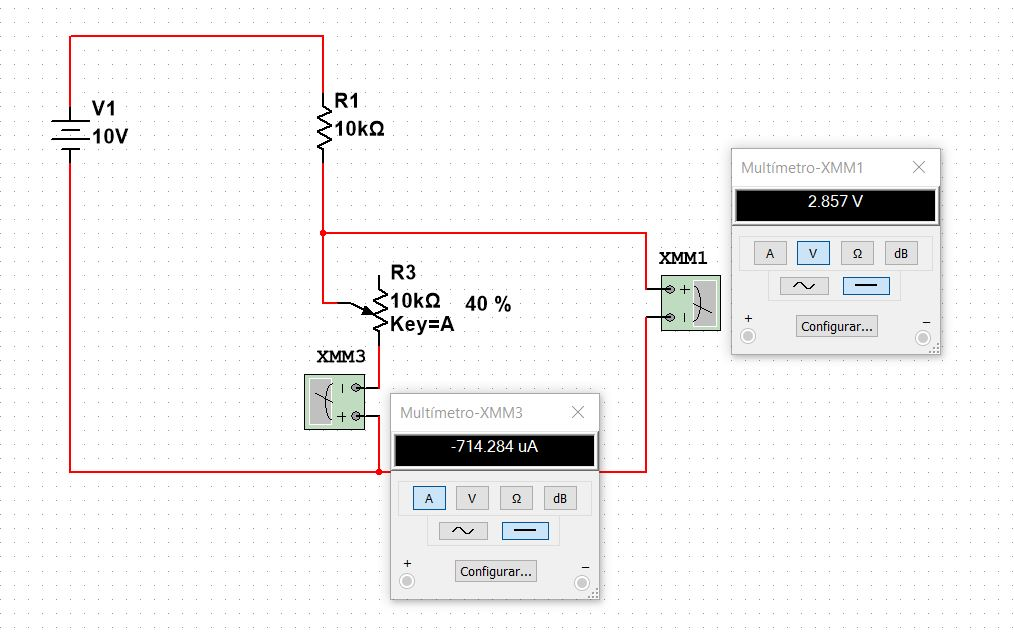
\includegraphics[scale=0.3]{imagenes1/2.4.JPG}
    \caption{Voltaje y resistencia de un potenciometro de 10 K$\Omega$ al 40\%}
    \label{fig:circuito3}
    \end{figure}
\newpage        
    \begin{figure}[h]
    \centering
    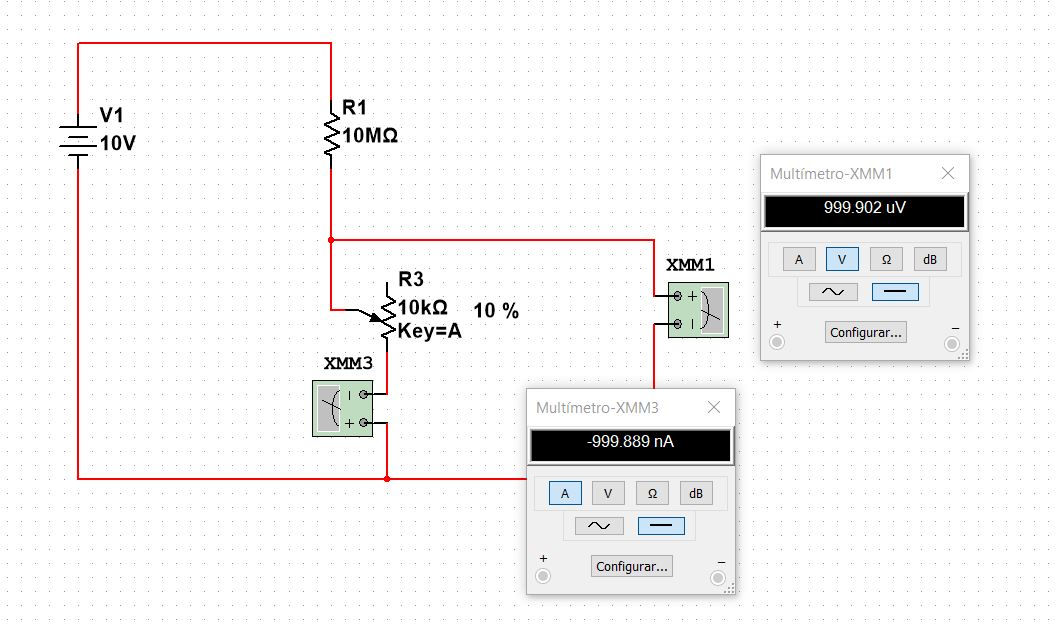
\includegraphics[scale=0.28]{imagenes1/2.5.JPG}
    \caption{Voltaje y resistencia de un potenciometro de 10 K$\Omega$ al 10\%}
    \label{fig:circuito4}
    \end{figure}

\item Simulación del paso 3
    \begin{figure}[h]
    \centering
    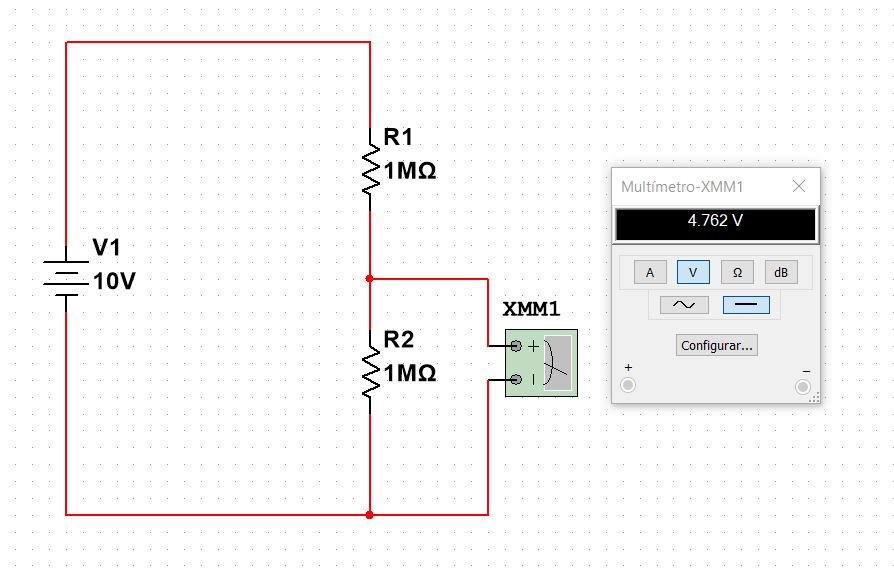
\includegraphics[scale=0.28]{imagenes1/3.JPG}
    \caption{Cálculo del voltaje BC para R_{1}=1 M$\Omega$ , R_{2}=1 M$\Omega$ , R_{v}=1 M$\Omega$ }
    \label{fig:circuito4}
    \end{figure}

\item Simulación del paso 4
    \begin{figure}[h]
    \centering
    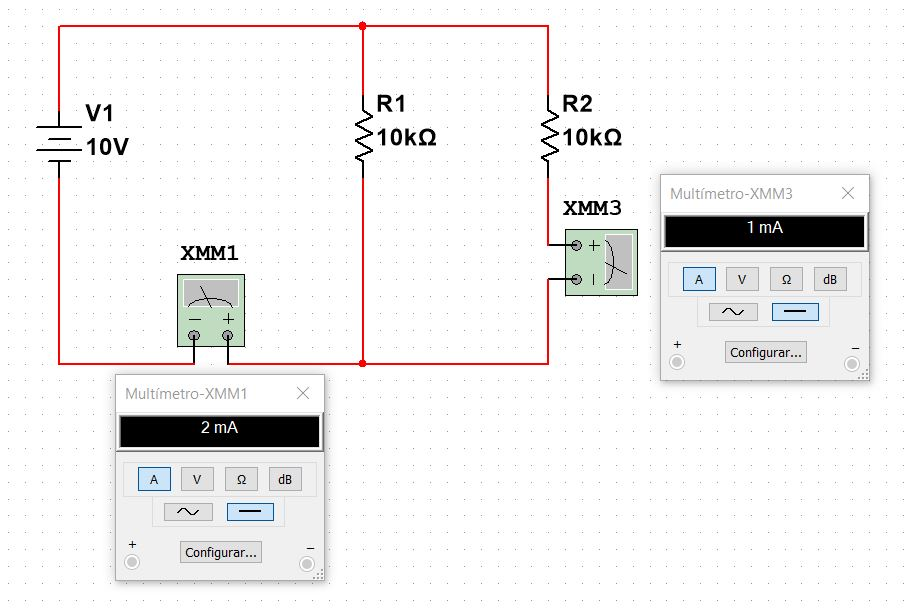
\includegraphics[scale=0.28]{imagenes1/4.1.JPG}
    \caption{Intensidad $I_{1}$ e $I_{2}$ , para el $R_{1}$=10 K$\Omega$, $R_{2}$ = 10 K$\Omega$ }
    \label{fig:circuito4}
    \end{figure}
\newpage   
    \begin{figure}[h]
    \centering
    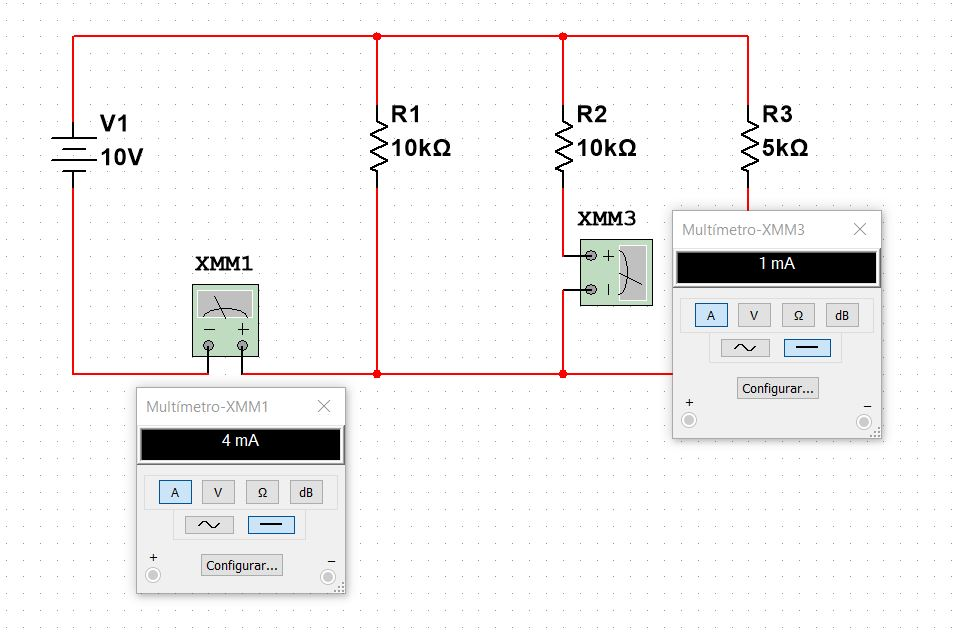
\includegraphics[scale=0.3]{imagenes1/4.2.JPG}
    \caption{Intensidad $I_{1}$ e $I_{2}$ , para el $R_{1}$=10 K$\Omega$, $R_{2}$ = 10 K$\Omega$ , R_{3}=5 K$\Omega$ }
    \label{fig:circuito4}
    \end{figure}
\item Simulación del paso 5    
    \begin{figure}[h]
    \centering
    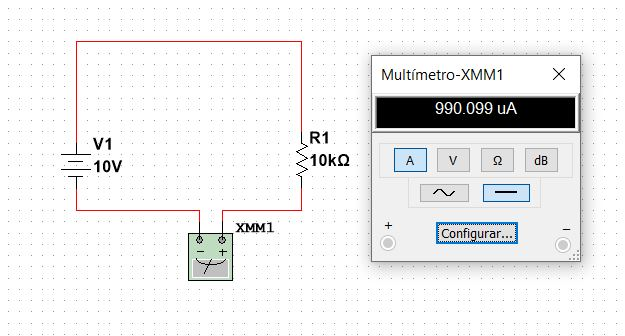
\includegraphics[scale=0.42]{imagenes1/5.1.JPG}
    \caption{Cálculo de intensidad para $R_{1}$ = 10 K$\Omega$ y $R_{A}$ = 100 $\Omega$ }
    \label{fig:circuito4}
    \end{figure}
    \begin{figure}[h]
    \centering
    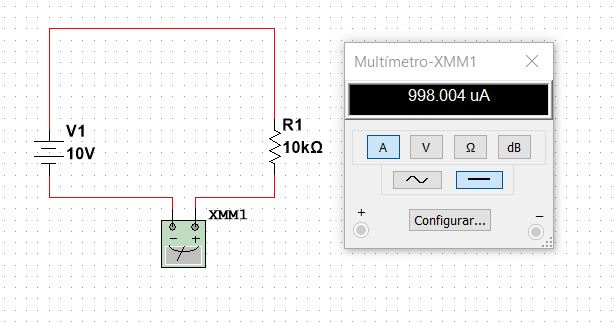
\includegraphics[scale=0.42]{imagenes1/5.2.JPG}
    \caption{Cálculo de intensidad para $R_{1}$ = 10 K$\Omega$ y $R_{A}$ = 20 $\Omega$  }
    \label{fig:circuito4}
    \end{figure}
\end{itemize}

\newpage
\section{Discusión de los resultados}
En el paso 1, no tuvimos problema entendiendo la funcionalidad de las bandas en resistencias y completando el cuadro, así como resolviendo el conjunto de resistencias.\\
En el paso 2, el valor de las resistencias y el voltaje fueron lo esperado. \\En el paso 3, usamos porcentajes diferentes no múltiplos entre sí para ser variados, y obtuvimos resultados satisfactorios.\\ En el paso 4, también la medida de las resistencias e intensidad de corriente fueron las esperadas.
\\En el paso 5, por trabajar con multimetros ideales, tambien obtuvimos resultados sin error relativo.

\section{Conclusiones}
\begin{itemize}
\item Pudimos poner a prueba la ley de ohm y kirchoff mediante experimentos sencillos, verificando su utilidad y eficacia.
\item Verificamos la utilidad de usar voltímetros y amperímetros ideales y de resistencias internas predeterminadas.
\item Aprendimos a utilizar instrumentos como el multímetro, el potenciómetro, así como armar circuitos con resistencias en serie y paralelo.
\end{itemize}

\section{Observaciones}
\begin{itemize}
\item Al tratar con herramientas e instrumentos ideales, el porcentaje de error relativo es nulo en todos los pasos, menos en el 3.
\item En los experimentos 2,4 y 5 tratamos la resistencia interna del multímetro como ideal , mientras que en el paso 3, fue de 1 M$\Omega$ .
\item El rango de medición del multímetro, en el paso 5, no afectó a los valores obtenidos.
\end{itemize}

%----------------------------------------------------------------------------------------
%	REFERENCE LIST
%----------------------------------------------------------------------------------------
\newpage
\begin{thebibliography}{99} % Bibliography - this is intentionally simple in this template

\bibitemCap 1 Guia para mediciones electrónicas.
Wolf – Smith, 1992, Prentice Hall
%\newblock Assortative pairing and life history strategy - a cross-cultural
%  study.
%\newblock {\em Human Nature}, 20:317--330.
 
\end{thebibliography}

%----------------------------------------------------------------------------------------


\end{document}
